\scanpage{70}
\mspage{69}

(25 \unsure{juin|Juin})

En dehors du cas quasi-ensembliste, je suspecte que la notion de support, telle qu'elle est présentée ici, est \unsure{cornée|cornue|connerie} --- qu'il ne faudrait parler de support d'une partie $A$ de $M$, disons, que quand les $X\in A$ sont mutuellement compatibles, ou du moins, si deux à deux ils admettent des subdivisions mutuellement compatibles. Voici un exemple typique.

\uline{Exemple} Stratos associé à un \deleted{segment}\inserted{ens.} ordonné $I$ (p.ex. un ``\uline{segment} ordonné'').
\[
M=M_0\amalg M_1
\]
$M_0$ (0-strates) $=\deleted{\unsure{I}}$\inserted{ens des parties \unsure{uniponctuelles} de $I$} $(=\operatorname{Drap}_0(I))$

% The following initial definition and its accompanying notes are cancelled together.
\deleted{$M_1$ (1-strates) $=\operatorname{Drap}_1(I)\simeq\{(a,b)\in I\times I\mid a<b\}$}
\inserted{\deleted{parties de $I$ de la forme $X_{ab}=\{x\mid a\leq x\leq b\}$ où $a<b$. Alors $a,b$ \unsure{uniquement déterminés}}}
\margin{\deleted{Pour $X\in M_1$ \unsure{défini} par $(a,b)$, on \unsure{écrira} $\partial X=\{a,b\}\subset M_0$. On}}
\[
\deleted{X\leq Y\quad\text{ssi}\quad X\subset Y\quad\text{donc}\quad
\left(\begin{gathered}X<Y\quad\text{ssi}\quad X\in M_1,\ Y\in M_1\\X\in\partial Y\end{gathered}\right)}
\]
\[
\deleted{X\ll Y\quad\text{ssi}\quad\{}
\]
% The opening brace above is abandoned on the manuscript; no condition is written after it.

$M_1$ (1-strates) $=$ ens des sous-segments de $I$, i.e. parties \inserted{$X$} de la forme $I_{a\leq\cdot\leq b}$, où $a<b$. (NB $a,b$ sont uniquement déterminés : origine et extrémité de $X$. On pose $\partial X=\{a,b\}$.

\[
X\leq Y\quad\Longleftrightarrow\quad
\left\{\begin{aligned}&X=Y\text{ ou}\\&X\in M_0,\ Y\in M_1,\quad X\in\partial\deleted{\unsure{X}}Y\end{aligned}\right.
\]
\margin{(dans ce cas, on écrit $X\triangleleft Y$\deleted{\unsure{ou} \unsure{l'inclusion} \unsure{d'incidence} $X\unsure{\triangleleft}Y$})}
\[
X\ll Y\quad\Longleftrightarrow\quad X\subset Y
\]
% The upward stroke at the replacement may be an insertion pointer rather than a quantifier.
\margin{($X\overset{\circ}{\ll}Y$ signifie $X\unsure{\ne}Y$ ou $\deleted{\unsure{X\triangleleft Y}}\inserted{\unsure{X\triangleleft Y|\nexists X\triangleleft Y}}$)}
\inserted{On est dans un des trois cas mutuellement exclusifs}
\[
X\unsure{\bowtie|\gtrless}Y\quad\Longleftrightarrow\quad
\left\{\begin{aligned}
&\text{\textcircled{a}}\ X=Y\quad\deleted{\text{ou}}\quad
\text{\textcircled{b}}\ X\in\partial Y\text{ ou }Y\in\partial X,\quad\deleted{\text{ou}}\\
&\qquad\text{(cas où }Y\text{ resp. }X\text{ est dans }M_1\text{).}\\
&\text{\textcircled{c}}\ \partial X\cup\partial Y,\ \text{tot. ordonné}\\
&\deleted{\unsure{X\cap Y=\varnothing|X\cup Y=\varnothing}}\\
&\deleted{\unsure{\partial X\cap Y|\partial X\cap\partial Y}}\\
&\text{et }X\cap Y\text{ est vide, ou réduit }\deleted{\unsure{X}}\inserted{\text{à}}\text{ un point, }\text{\uline{d'où}}
\end{aligned}\right.
\]
on est dans un des cas : $\alpha)$ $\exists a\leq b<c\leq d$ avec $X=[a,b]$, $Y=[c,d]$ \inserted{ou l'inverse} ou $\beta)$ $\exists a<b<c$ avec $X=[a,b]$, $Y=[\unsure{b},\unsure{c}]$ ou l'inverse.

\figure{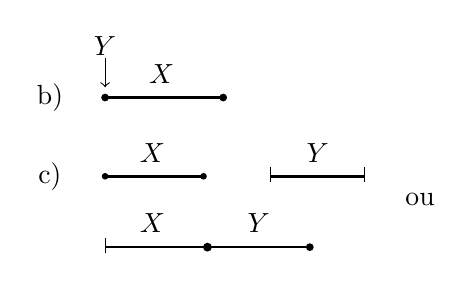
\begin{tikzpicture}[x=1cm,y=1cm]
\node at (-0.7,1.9) {b)};
\draw[line width=0.9pt] (0,1.9)--(1.5,1.9);
\fill (0,1.9) circle (1.4pt);
\fill (1.5,1.9) circle (1.4pt);
\node at (0.72,2.2) {$X$};
\node at (0,2.55) {$Y$};
\draw[->] (0,2.4)--(0,2.03);
\node at (-0.7,0.9) {c)};
\draw[line width=0.9pt] (0,0.9)--(1.25,0.9);
\fill (0,0.9) circle (1.2pt);
\fill (1.25,0.9) circle (1.2pt);
\node at (0.6,1.2) {$X$};
\draw[line width=0.9pt] (2.1,0.9)--(3.3,0.9);
\draw (2.1,0.83)--(2.1,1.02) (3.3,0.83)--(3.3,1.02);
\node at (2.7,1.2) {$Y$};
\node at (4,0.6) {ou};
\draw[line width=0.9pt] (0,0)--(2.6,0);
\draw (0,-0.08)--(0,0.12);
\fill (1.3,0) circle (1.6pt);
\fill (2.6,0) circle (1.4pt);
\node at (0.6,0.3) {$X$};
\node at (1.95,0.3) {$Y$};
\end{tikzpicture}}

\uline{NB}. Tous les axiomes sont satisfaits, à l'exception de $\mathrm{AtL1}$ (\unsure{divisibilité}), satisfait \unsure{ssi|ss} les intervalles $]a,b[$ sont $\ne\varnothing$ $(a<b)$.
